\documentclass[aspectratio=169]{beamer}
\usetheme{FLUKA}
\usepackage[utf8]{inputenc}
\usepackage[english]{babel}
\usepackage[T1]{fontenc}

\usepackage{pgfplots} % for tikz images
\pgfmathdeclarefunction{gauss}{2}{%
  \pgfmathparse{1/(#2*sqrt(2*pi))*exp(-((x-#1)^2)/(2*#2^2))}%
}

% remove if you do not need them
\usetikzlibrary{calc,positioning}

\title{Your lecture title}

\subtitle{23rd FLUKA Beginner's Course \\ Lanzhou University, \\ Lanzhou, China}
\date{June 2--7, 2024}

% Fill the author/institute even though they are currently not shown in the slides
\author{Your Name}
\institute[Your Short Institute]{Your Full Institute}

\AtBeginSection[]{%
  \begin{frame}<beamer>{Outline}
    \tableofcontents[currentsection]
  \end{frame}
}

\begin{document}

\begin{frame}[plain]
\maketitle
\end{frame}

\begin{frame}{Outline}
\tableofcontents
\end{frame}

\section{Colours}

\begin{frame}{\secname}{https://nemo.kiwi/latex/colors.html}
  \centering
  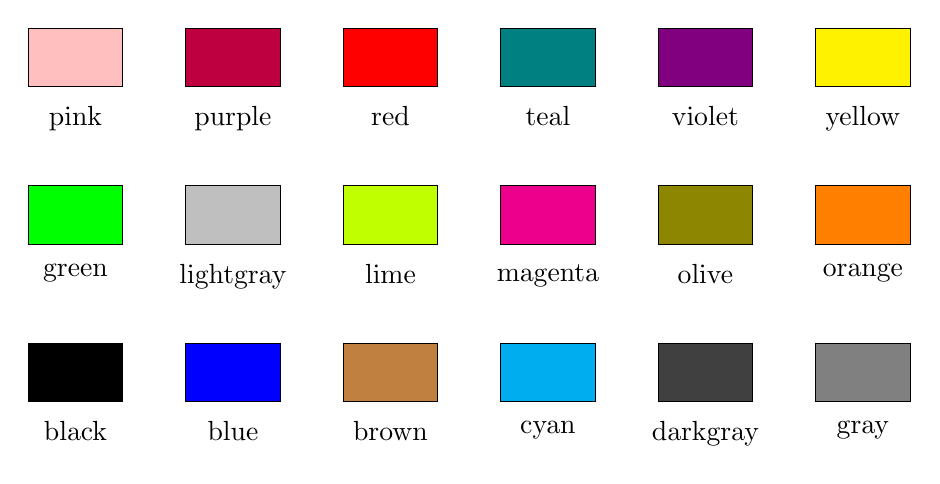
\begin{tikzpicture}
    \def \nColumns {6};
    \def \baseWidth {0.6cm};
    \def \baseHeight {0.37267081cm};

    \foreach \color [count=\i from 0] in {black, blue, brown, cyan, darkgray, gray,
      green, lightgray, lime, magenta, olive,
      orange, pink, purple, red, teal, violet,
      yellow} {
      \coordinate (center_\color)
      at ({2*mod(\i, \nColumns)}, {2*div(\i, \nColumns)});
      \coordinate (rectangle_bottom_\color)
      at ($(center_\color) - (\baseWidth, \baseHeight)$);
      \coordinate (rectangle_top_\color)
      at ($(center_\color) + (\baseWidth, \baseHeight)$);

      \draw[fill=\color, black] (rectangle_bottom_\color) rectangle (rectangle_top_\color);
      \node[below=0.5cm of center_\color] {\color};
    }
  \end{tikzpicture}
\end{frame}

 \section{Equation}
 \begin{frame}{\secname}
   \centering
   \Huge
   $$
   u(\rho,t) = J_0(k\rho) \cos(2\pi f t)
   $$
 \end{frame}

 \section{Matrix}
 \begin{frame}{\secname}
   \centering
   \Huge
   $$
   \mu = \left(
     \begin{array}{ccc}
       \mu_{1} & -jk & 0 \\
       jk & \mu_{1} & 0 \\
       0 & 0 & 1
     \end{array}
   \right)
   $$
 \end{frame}

\section{Examples}
 \begin{frame}{\secname}
   \only<1>{
     \framesubtitle{Enumerate}
     \begin{enumerate}
     \item en
     \item tv\aa
     \item tre
     \end{enumerate}
   }
   \only<2>{
     \framesubtitle{Itemize}
     \begin{itemize}
     \item tro
     \item hopp
     \item k\"arlek
     \end{itemize}
   }
   \only<3>{
     \framesubtitle{Block}
     \begin{block}{Block title}
       text inside block
     \end{block}
   }
   \only<4>{
     \framesubtitle{Example}
     \begin{example}
       text inside example
     \end{example}
   }
   \only<5>{
     \framesubtitle{Quote}
     \begin{exampleblock}{}
       ``The first principle is that you must not fool yourself~--- and you are the easiest person to fool.''
       \vskip 5mm
       \hspace*\fill{\small--- Richard Feynman}
     \end{exampleblock}
   }
   \only<6>{
     \framesubtitle{Table}
     \centering
     \begin{tabular}{ccc}
       \toprule
        $A$ & $B$ & $A\mathbin{\oplus}B$ \\
       \midrule
       0 & 0 & 0 \\
       0 & 1 & 1 \\
       1 & 0 & 1 \\
       1 & 1 & 0 \\
       \bottomrule
      \end{tabular}
   }
   \only<7>{
     \framesubtitle{TikZ picture}
     \centering
     \begin{tikzpicture}
       \begin{axis}[every axis plot post/.append style={mark=none,domain=-2:3,samples=50,smooth},
         axis x line*=bottom,
         axis y line*=left,
         enlargelimits=upper,
         xlabel=$x$,
         ylabel=$y$]
         \addplot+[ultra thick] {gauss(0,0.5)};
         \addplot+[ultra thick] {gauss(1,0.75)};
       \end{axis}
     \end{tikzpicture}
   }
   \only<8>{
     \framesubtitle{External graphics}
     \begin{block}{Heavy ion incident onto ATIC spectrometer}
       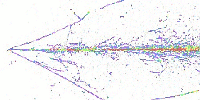
\includegraphics[width=0.49\linewidth]{figs/g1-soft.png} \hfill
       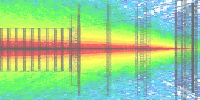
\includegraphics[width=0.49\linewidth]{figs/g5-soft.png}

       \hfill\copyr{http://www.fluka.org}{Toni Empl}
     \end{block}
   }
 \end{frame}

 \section{Bibliography}
 \begin{frame}{\secname}
   \begin{thebibliography}{3}
     \beamertemplatearticlebibitems
   \bibitem{Tantau2010}
     Till Tantau, Joseph Wright, Vedran Mileti\'c
     \newblock The BEAMER class User Guide
     \newblock \href{http://bitbucket.org/rivanvx/beamer}{http://bitbucket.org/rivanvx/beamer}
     \newblock 2010

     \beamertemplatebookbibitems
   \bibitem{Book}
     Book author
     \newblock{Book title}
     \newblock{Year}
   \end{thebibliography}
 \end{frame}

 \finalpage
\end{document}
